\subsection{Experimental Results}

\looseness=-1

We compare the performance of SynEnum and SynMS under the normal and mis\`{e}re rules, respectively.

The latest experimental data are taken from Sheet1 of the corresponding report workbooks, and the running-time curves are generated from the summary data filtered by the Sheet1 counts.

In each table, the column ``Solved'' denotes the number of test cases solved by each approach.

The columns ``Time'' and ``Size'' denote the average running time and average solution size over the solved test cases for each approach.

The optimal data of each group are in bold.

\subsubsection{Experimental Results under normal rule}

\textbf{Comparison on Subtraction game.}
Table \ref{tab:normal-sub-winFormulas} presents the results for synthesizing winning formulas in the Subtraction game under the normal rule.
Out of $479$ test cases, SynEnum solves $136$ formula cases, while SynMS solves $467$, with success rates of $28.4\%$ and $97.5\%$, respectively.
Thus SynMS solves $331$ more formula cases than SynEnum.
The average formula synthesis time is $8.77$ seconds for SynEnum and $52.06$ seconds for SynMS.
Table \ref{tab:normal-sub-winStrategies} summarizes the corresponding results for synthesizing winning strategies.
SynEnum solves $136$ strategy cases, whereas SynMS solves $466$ strategy cases.
This gives SynMS an advantage of $330$ strategy cases in this benchmark group.
The average strategy synthesis time is $1.04$ seconds for SynEnum and $14.54$ seconds for SynMS.
In terms of solution size, SynEnum produces smaller formulas and strategies on average, with average sizes $13.30$ and $60.24$, while SynMS has average sizes $33.05$ and $118.54$.
Figure \ref{fig:normal-sub-line} shows the cumulative number of solved test cases over time after filtering the summary data according to the latest Sheet1 counts.

\begin{table*}[h!]
	%字体大小和行距
	\footnotesize
	%列距
	\setlength{\tabcolsep}{2pt}
	\centering
	\begin{tabular}{|c|c|c|c|c|c|c|c|}
		\hline
		\multirow{3}{*}{Category} & \multirow{3}*{\tabincell{c}{Test \\ cases}} & \multicolumn{6}{c|}{Formula}  \\ \cline{3-8} &  & \multicolumn{2}{c|}{Solved} & \multicolumn{2}{c|}{Time} & \multicolumn{2}{c|}{Size} \\ \cline{3-8} & & \multicolumn{1}{c|}{SynEnum} & \multicolumn{1}{c|}{SynMS} & \multicolumn{1}{c|}{SynEnum} & \multicolumn{1}{c|}{SynMS} & \multicolumn{1}{c|}{SynEnum} & SynMS \\ \hline
		Take-away & 30 & \textbf{30} & \textbf{30} & 6.77 & \textbf{6.11} & \textbf{3.00} & \textbf{3.00} \\ \hline
		Subtraction & 385 & 98 & \textbf{382} & \textbf{6.91} & 37.85 & \textbf{14.21} & 34.84 \\ \hline
		$S,D$-Mark & 64 & 8 & \textbf{55} & \textbf{101.97} & 175.77 & \textbf{10.00} & 36.96 \\ \hline
		Total & 479 & 136 & \textbf{467} & \textbf{8.77} & 52.06 & \textbf{13.30} & 33.05 \\ \hline
	\end{tabular}
	\caption{Results of synthesizing winning formulas for Sub games under normal rule}
	\label{tab:normal-sub-winFormulas}
\end{table*}

\begin{table*}[h!]
	%字体大小和行距
	\footnotesize
	%列距
	\setlength{\tabcolsep}{2pt}
	\centering
	\begin{tabular}{|c|c|c|c|c|c|c|c|}
		\hline
		\multirow{3}{*}{Category} & \multirow{3}*{\tabincell{c}{Test \\ cases}} & \multicolumn{6}{c|}{Strategy}  \\ \cline{3-8} &  & \multicolumn{2}{c|}{Solved} & \multicolumn{2}{c|}{Time} & \multicolumn{2}{c|}{Size} \\ \cline{3-8} & & \multicolumn{1}{c|}{SynEnum} & \multicolumn{1}{c|}{SynMS} & \multicolumn{1}{c|}{SynEnum} & \multicolumn{1}{c|}{SynMS} & \multicolumn{1}{c|}{SynEnum} & SynMS \\ \hline
		Take-away & 30 & \textbf{30} & \textbf{30} & 9.22 & \textbf{7.64} & \textbf{93.00} & \textbf{93.00} \\ \hline
		Subtraction & 385 & 98 & \textbf{382} & \textbf{0.39} & 0.61 & \textbf{57.73} & 121.80 \\ \hline
		$S,D$-Mark & 64 & 8 & \textbf{54} & \textbf{0.46} & 116.93 & \textbf{53.00} & 109.70 \\ \hline
		Total & 479 & 136 & \textbf{466} & \textbf{1.04} & 14.54 & \textbf{60.24} & 118.54 \\ \hline
	\end{tabular}
	\caption{Results of synthesizing winning strategies for Sub games under normal rule}
	\label{tab:normal-sub-winStrategies}
\end{table*}

\begin{figure}[h!]
    \centering
    \begin{subfigure}[b]{0.49\textwidth}
        \centering
        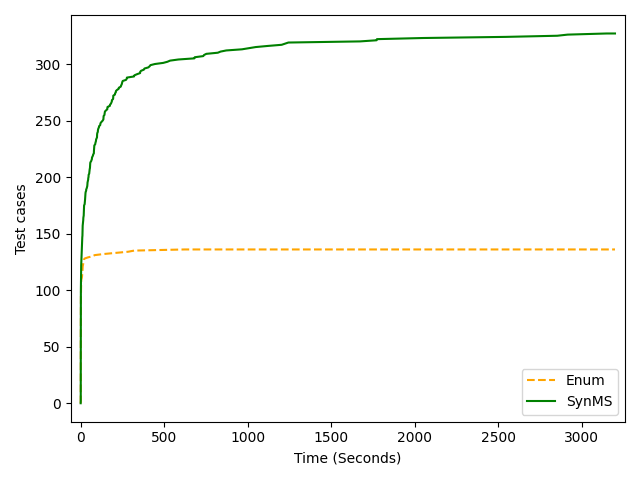
\includegraphics[width=\textwidth]{fig/normal-sub-f.png}
        \caption{Comparison on synthesizing winning formulas on the whole benchmark}
    \end{subfigure}
    \begin{subfigure}[b]{0.49\textwidth}
        \centering
        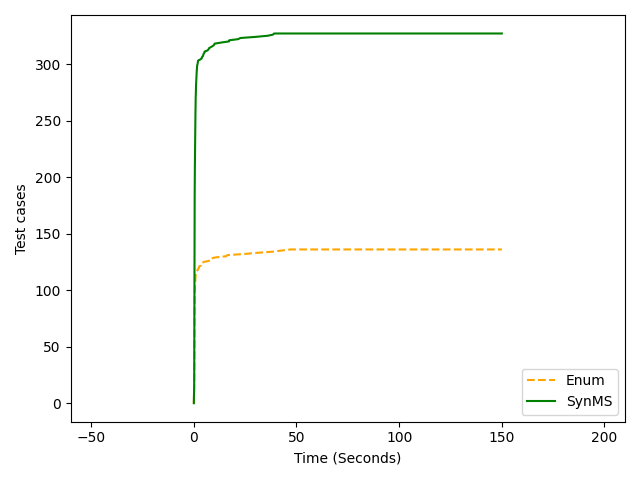
\includegraphics[width=\textwidth]{fig/normal-sub-s.png}
        \caption{Comparison on synthesizing winning strategies on the whole benchmark}
    \end{subfigure}
    \caption{Comparison of the running time of synthesizing winning formula and strategy for Subtraction game under normal rule}
    \label{fig:normal-sub-line}
\end{figure}

\textbf{Comparison on Nim game.}
Table \ref{tab:normal-nim-winFormulas} presents the results for synthesizing winning formulas in the Nim game under the normal rule.
Out of $302$ test cases, SynEnum solves $62$ formula cases, while SynMS solves $95$, with success rates of $20.5\%$ and $31.5\%$, respectively.
Thus SynMS solves $33$ more formula cases than SynEnum.
The average formula synthesis time is $9.77$ seconds for SynEnum and $5.70$ seconds for SynMS.
Table \ref{tab:normal-nim-winStrategies} summarizes the corresponding results for synthesizing winning strategies.
SynEnum solves $59$ strategy cases, whereas SynMS solves $86$ strategy cases.
This gives SynMS an advantage of $27$ strategy cases in this benchmark group.
The average strategy synthesis time is $44.60$ seconds for SynEnum and $63.38$ seconds for SynMS.
In terms of solution size, SynEnum produces smaller formulas and strategies on average, with average sizes $5.77$ and $28.63$, while SynMS has average sizes $71.34$ and $481.79$.
Figure \ref{fig:normal-nim-line} shows the cumulative number of solved test cases over time after filtering the summary data according to the latest Sheet1 counts.

\begin{table*}[h!]
	%字体大小和行距
	\scriptsize
	%列距
	\setlength{\tabcolsep}{1pt}
	\centering
	\begin{tabular}{|c|c|c|c|c|c|c|c|}
		\hline
		\multirow{3}{*}{Category} & \multirow{3}*{\tabincell{c}{Test \\ cases}} & \multicolumn{6}{c|}{Formula}  \\ \cline{3-8} &  & \multicolumn{2}{c|}{Solved} & \multicolumn{2}{c|}{Time} & \multicolumn{2}{c|}{Size} \\ \cline{3-8} & & \multicolumn{1}{c|}{SynEnum} & \multicolumn{1}{c|}{SynMS} & \multicolumn{1}{c|}{SynEnum} & \multicolumn{1}{c|}{SynMS} & \multicolumn{1}{c|}{SynEnum} & SynMS \\ \hline
		Nim & 7 & 1 & \textbf{2} & \textbf{1.13} & 3.66 & \textbf{4.00} & 23.50 \\ \hline
		Monotonic Nim & 7 & \textbf{7} & \textbf{7} & \textbf{0.94} & 1.28 & 4.86 & \textbf{3.86} \\ \hline
		Empty and Transfer & 7 & \textbf{2} & 1 & \textbf{2.83} & 2.98 & \textbf{7.50} & 18.00 \\ \hline
		Empty All But One & 6 & \textbf{6} & \textbf{6} & 24.40 & \textbf{4.64} & \textbf{5.33} & 32.00 \\ \hline
		Empty and Redistribute & 6 & 1 & \textbf{2} & 36.61 & \textbf{2.65} & \textbf{13.00} & 178.00 \\ \hline
		Entropy Reduction Game & 7 & \textbf{1} & \textbf{1} & \textbf{12.63} & 19.53 & \textbf{8.00} & 12.00 \\ \hline
		Min Game & 6 & 1 & \textbf{3} & \textbf{3.10} & 8.95 & \textbf{6.00} & 117.67 \\ \hline
		$l$-Slow Nim & 180 & 9 & \textbf{11} & \textbf{1.42} & 7.19 & \textbf{4.89} & 135.09 \\ \hline
		Sharing Nim & 7 & 4 & \textbf{6} & \textbf{4.78} & 6.31 & \textbf{5.00} & 10.83 \\ \hline
		Small Nim & 7 & \textbf{7} & \textbf{7} & 18.29 & \textbf{1.70} & \textbf{7.29} & 11.86 \\ \hline
		Greedy Nim & 7 & 2 & \textbf{7} & 6.92 & \textbf{5.47} & \textbf{8.50} & 159.86 \\ \hline
		Odd-or-Even Nim & 7 & 2 & \textbf{6} & 3.88 & \textbf{3.28} & \textbf{7.00} & 230.83 \\ \hline
		Modular Nim & 5 & 1 & \textbf{2} & \textbf{1.12} & 1.94 & \textbf{4.00} & 30.00 \\ \hline
		Pointed Nim & 7 & 1 & \textbf{7} & 23.07 & \textbf{9.84} & \textbf{4.00} & 49.29 \\ \hline
		End Nim & 7 & 1 & \textbf{7} & \textbf{1.08} & 2.48 & \textbf{4.00} & 107.71 \\ \hline
		Loop End Nim & 7 & 2 & \textbf{7} & 78.32 & \textbf{13.02} & \textbf{9.50} & 51.86 \\ \hline
		Staircase Nim & 7 & \textbf{7} & \textbf{7} & \textbf{1.79} & 2.52 & 3.71 & \textbf{2.86} \\ \hline
		Circular Nim & 15 & \textbf{7} & 6 & \textbf{2.52} & 9.58 & \textbf{6.14} & 15.33 \\ \hline
		Total & 302 & 62 & \textbf{95} & 9.77 & \textbf{5.70} & \textbf{5.77} & 71.34 \\ \hline
	\end{tabular}
	\caption{Results of synthesizing winning formulas for Nim games under normal rule}
	\label{tab:normal-nim-winFormulas}
\end{table*}

\begin{table*}[h!]
	%字体大小和行距
	\scriptsize
	%列距
	\setlength{\tabcolsep}{1pt}
	\centering
	\begin{tabular}{|c|c|c|c|c|c|c|c|}
		\hline
		\multirow{3}{*}{Category} & \multirow{3}*{\tabincell{c}{Test \\ cases}} & \multicolumn{6}{c|}{Strategy}  \\ \cline{3-8} &  & \multicolumn{2}{c|}{Solved} & \multicolumn{2}{c|}{Time} & \multicolumn{2}{c|}{Size} \\ \cline{3-8} & & \multicolumn{1}{c|}{SynEnum} & \multicolumn{1}{c|}{SynMS} & \multicolumn{1}{c|}{SynEnum} & \multicolumn{1}{c|}{SynMS} & \multicolumn{1}{c|}{SynEnum} & SynMS \\ \hline
		Nim & 7 & 1 & \textbf{2} & 1.12 & \textbf{0.17} & \textbf{12.00} & 54.00 \\ \hline
		Monotonic Nim & 7 & \textbf{7} & \textbf{7} & 1.16 & \textbf{0.09} & 28.86 & \textbf{22.86} \\ \hline
		Empty and Transfer & 7 & \textbf{2} & 1 & \textbf{0.78} & 9.61 & 18.00 & \textbf{12.00} \\ \hline
		Empty All But One & 6 & \textbf{6} & \textbf{6} & \textbf{7.47} & 16.22 & \textbf{5.33} & \textbf{5.33} \\ \hline
		Empty and Redistribute & 6 & 0 & \textbf{1} & - & 24.35 & - & 9.00 \\ \hline
		Entropy Reduction Game & 7 & 0 & \textbf{1} & - & 4.08 & - & 112.00 \\ \hline
		Min Game & 6 & 1 & \textbf{3} & \textbf{0.46} & 45.96 & \textbf{11.00} & 3216.33 \\ \hline
		$l$-Slow Nim & 180 & 9 & \textbf{11} & \textbf{0.49} & 38.37 & \textbf{30.89} & 821.09 \\ \hline
		Sharing Nim & 7 & 3 & \textbf{6} & \textbf{0.44} & 35.95 & \textbf{22.33} & 1234.50 \\ \hline
		Small Nim & 7 & \textbf{7} & \textbf{7} & 2.72 & \textbf{1.25} & 72.57 & \textbf{30.86} \\ \hline
		Greedy Nim & 7 & 2 & \textbf{5} & \textbf{1.49} & 282.73 & \textbf{49.50} & 1101.40 \\ \hline
		Odd-or-Even Nim & 7 & 2 & \textbf{6} & \textbf{0.89} & 259.60 & \textbf{16.50} & 859.83 \\ \hline
		Modular Nim & 5 & 1 & \textbf{2} & \textbf{0.51} & 2.15 & \textbf{14.00} & 55.00 \\ \hline
		Pointed Nim & 7 & 1 & \textbf{7} & 0.74 & \textbf{0.53} & \textbf{8.00} & 11.43 \\ \hline
		End Nim & 7 & 1 & \textbf{4} & \textbf{1.08} & 147.56 & \textbf{8.00} & 336.75 \\ \hline
		Loop End Nim & 7 & 2 & \textbf{7} & \textbf{1.24} & 109.37 & \textbf{25.00} & 335.86 \\ \hline
		Staircase Nim & 7 & \textbf{7} & \textbf{7} & 2.06 & \textbf{0.07} & 23.71 & \textbf{17.43} \\ \hline
		Circular Nim & 15 & \textbf{7} & 3 & 360.97 & \textbf{64.87} & 23.57 & \textbf{7.00} \\ \hline
		Total & 302 & 59 & \textbf{86} & \textbf{44.60} & 63.38 & \textbf{28.63} & 481.79 \\ \hline
	\end{tabular}
	\caption{Results of synthesizing winning strategies for Nim games under normal rule}
	\label{tab:normal-nim-winStrategies}
\end{table*}

\begin{figure}[h!]
    \centering
    \begin{subfigure}[b]{0.49\textwidth}
        \centering
        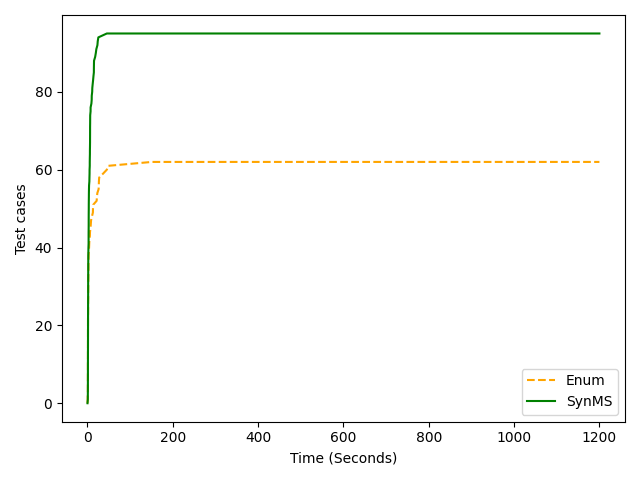
\includegraphics[width=\textwidth]{fig/normal-nim-f.png}
        \caption{Comparison on synthesizing winning formulas on the whole benchmark}
    \end{subfigure}
    \begin{subfigure}[b]{0.49\textwidth}
        \centering
        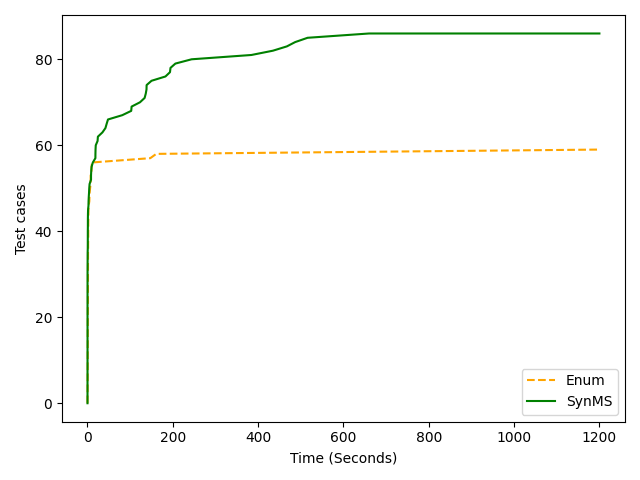
\includegraphics[width=\textwidth]{fig/normal-nim-s.png}
        \caption{Comparison on synthesizing winning strategies on the whole benchmark}
    \end{subfigure}
    \caption{Comparison of the running time of synthesizing winning formula and strategy for Nim game under normal rule}
    \label{fig:normal-nim-line}
\end{figure}

\textbf{Comparison on Welter game.}
Table \ref{tab:normal-welter-winFormulas} presents the results for synthesizing winning formulas in the Welter game under the normal rule.
Out of $7$ test cases, SynEnum solves $4$ formula cases, while SynMS solves $5$, with success rates of $57.1\%$ and $71.4\%$, respectively.
Thus SynMS solves $1$ more formula cases than SynEnum.
The average formula synthesis time is $50.05$ seconds for SynEnum and $3.50$ seconds for SynMS.
Table \ref{tab:normal-welter-winStrategies} summarizes the corresponding results for synthesizing winning strategies.
SynEnum solves $4$ strategy cases, whereas SynMS solves $5$ strategy cases.
This gives SynMS an advantage of $1$ strategy cases in this benchmark group.
The average strategy synthesis time is $1.08$ seconds for SynEnum and $0.55$ seconds for SynMS.
In terms of solution size, SynEnum produces smaller formulas and strategies on average, with average sizes $7.20$ and $43.20$, while SynMS has average sizes $74.40$ and $399.20$.
Figure \ref{fig:normal-welter-line} shows the cumulative number of solved test cases over time after filtering the summary data according to the latest Sheet1 counts.

\begin{table*}[h!]
	%字体大小和行距
	\footnotesize
	%列距
	\setlength{\tabcolsep}{3pt}
	\centering
	\begin{tabular}{|c|c|c|c|c|c|c|c|}
		\hline
		\multirow{3}{*}{Category} & \multirow{3}*{\tabincell{c}{Test \\ cases}} & \multicolumn{6}{c|}{Formula}  \\ \cline{3-8} &  & \multicolumn{2}{c|}{Solved} & \multicolumn{2}{c|}{Time} & \multicolumn{2}{c|}{Size} \\ \cline{3-8} & & \multicolumn{1}{c|}{SynEnum} & \multicolumn{1}{c|}{SynMS} & \multicolumn{1}{c|}{SynEnum} & \multicolumn{1}{c|}{SynMS} & \multicolumn{1}{c|}{SynEnum} & SynMS \\ \hline
		Welter & 1 & \textbf{1} & \textbf{1} & 123.22 & \textbf{3.00} & \textbf{12.00} & 36.00 \\ \hline
		$l$-Welter & 5 & 2 & \textbf{3} & \textbf{1.38} & 4.35 & \textbf{4.00} & 100.00 \\ \hline
		Max-Welter & 1 & \textbf{1} & \textbf{1} & 122.86 & \textbf{1.46} & \textbf{12.00} & 36.00 \\ \hline
		Total & 7 & 4 & \textbf{5} & 50.05 & \textbf{3.50} & \textbf{7.20} & 74.40 \\ \hline
	\end{tabular}
	\caption{Results of synthesizing winning formulas for Welter games under normal rule}
	\label{tab:normal-welter-winFormulas}
\end{table*}

\begin{table*}[h!]
	%字体大小和行距
	\footnotesize
	%列距
	\setlength{\tabcolsep}{3pt}
	\centering
	\begin{tabular}{|c|c|c|c|c|c|c|c|}
		\hline
		\multirow{3}{*}{Category} & \multirow{3}*{\tabincell{c}{Test \\ cases}} & \multicolumn{6}{c|}{Strategy}  \\ \cline{3-8} &  & \multicolumn{2}{c|}{Solved} & \multicolumn{2}{c|}{Time} & \multicolumn{2}{c|}{Size} \\ \cline{3-8} & & \multicolumn{1}{c|}{SynEnum} & \multicolumn{1}{c|}{SynMS} & \multicolumn{1}{c|}{SynEnum} & \multicolumn{1}{c|}{SynMS} & \multicolumn{1}{c|}{SynEnum} & SynMS \\ \hline
		Welter & 1 & \textbf{1} & \textbf{1} & 1.75 & \textbf{0.23} & 44.00 & \textbf{38.00} \\ \hline
		$l$-Welter & 5 & 2 & \textbf{3} & \textbf{0.56} & 0.78 & \textbf{40.00} & 637.33 \\ \hline
		Max-Welter & 1 & \textbf{1} & \textbf{1} & 1.96 & \textbf{0.17} & 52.00 & \textbf{46.00} \\ \hline
		Total & 7 & 4 & \textbf{5} & 1.08 & \textbf{0.55} & \textbf{43.20} & 399.20 \\ \hline
	\end{tabular}
	\caption{Results of synthesizing winning strategies for Welter games under normal rule}
	\label{tab:normal-welter-winStrategies}
\end{table*}

\begin{figure}[h!]
    \centering
    \begin{subfigure}[b]{0.49\textwidth}
        \centering
        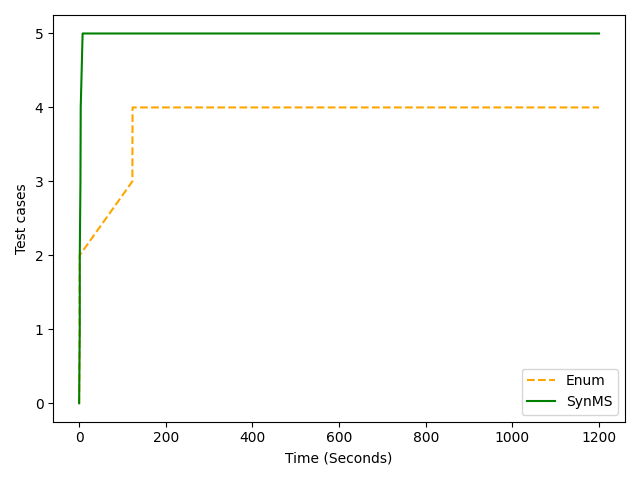
\includegraphics[width=\textwidth]{fig/normal-welter-f.png}
        \caption{Comparison on synthesizing winning formulas on the whole benchmark}
    \end{subfigure}
    \begin{subfigure}[b]{0.49\textwidth}
        \centering
        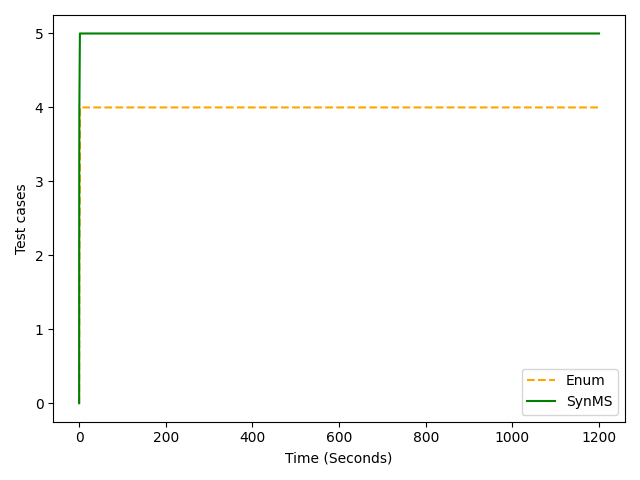
\includegraphics[width=\textwidth]{fig/normal-welter-s.png}
        \caption{Comparison on synthesizing winning strategies on the whole benchmark}
    \end{subfigure}
    \caption{Comparison of the running time of synthesizing winning formula and strategy for Welter game under normal rule}
    \label{fig:normal-welter-line}
\end{figure}

\textbf{Comparison on Wythoff game.}
Table \ref{tab:normal-wythoff-winFormulas} presents the results for synthesizing winning formulas in the Wythoff game under the normal rule.
Out of $2924$ test cases, SynEnum solves $1863$ formula cases, while SynMS solves $2679$, with success rates of $63.7\%$ and $91.6\%$, respectively.
Thus SynMS solves $816$ more formula cases than SynEnum.
The average formula synthesis time is $26.10$ seconds for SynEnum and $15.29$ seconds for SynMS.
Table \ref{tab:normal-wythoff-winStrategies} summarizes the corresponding results for synthesizing winning strategies.
SynEnum solves $1815$ strategy cases, whereas SynMS solves $2200$ strategy cases.
This gives SynMS an advantage of $385$ strategy cases in this benchmark group.
The average strategy synthesis time is $2.27$ seconds for SynEnum and $246.62$ seconds for SynMS.
In terms of solution size, SynEnum produces smaller formulas and strategies on average, with average sizes $5.67$ and $40.96$, while SynMS has average sizes $44.80$ and $380.59$.
Figure \ref{fig:normal-wythoff-line} shows the cumulative number of solved test cases over time after filtering the summary data according to the latest Sheet1 counts.

\begin{table*}[h!]
	%字体大小和行距
	\fontsize{4}{8}
	\selectfont
	%列距
	\setlength{\tabcolsep}{0.8pt}
	\centering
	\begin{tabular}{|c|c|c|c|c|c|c|c|}
		\hline
		\multirow{3}{*}{Category} & \multirow{3}*{\tabincell{c}{Test \\ cases}} & \multicolumn{6}{c|}{Formula}  \\ \cline{3-8} &  & \multicolumn{2}{c|}{Solved} & \multicolumn{2}{c|}{Time} & \multicolumn{2}{c|}{Size} \\ \cline{3-8} & & \multicolumn{1}{c|}{SynEnum} & \multicolumn{1}{c|}{SynMS} & \multicolumn{1}{c|}{SynEnum} & \multicolumn{1}{c|}{SynMS} & \multicolumn{1}{c|}{SynEnum} & SynMS \\ \hline
		Wythoff & 21 & 13 & \textbf{19} & 11.18 & \textbf{2.44} & \textbf{5.77} & 49.95 \\ \hline
		$l$-Wythoff & 140 & 93 & \textbf{120} & \textbf{25.64} & 40.09 & \textbf{6.45} & 63.65 \\ \hline
		Monotonic $l$-Diet Wythoff & 105 & 81 & \textbf{103} & 13.69 & \textbf{6.39} & \textbf{5.49} & 78.92 \\ \hline
		Wythoff with subtraction set $S$ & 315 & 177 & \textbf{287} & 20.20 & \textbf{2.84} & \textbf{5.65} & 55.32 \\ \hline
		Wythoff with a function $f$ & 168 & 118 & \textbf{154} & 16.44 & \textbf{4.71} & \textbf{5.59} & 47.68 \\ \hline
		1st($l_1$,$l_2$)\-restricted Wythoff & 315 & 119 & \textbf{285} & 27.18 & \textbf{2.26} & \textbf{5.95} & 57.56 \\ \hline
		2nd($l_1$,$l_2$)\-restricted Wythoff & 600 & 543 & \textbf{600} & 29.32 & \textbf{2.12} & \textbf{4.83} & 24.04 \\ \hline
		3rd($l_1$,$l_2$)\-restricted Wythoff & 700 & 392 & \textbf{578} & \textbf{37.42} & 50.54 & \textbf{6.52} & 50.73 \\ \hline
		4th($l_1$,$l_2$)\-restricted Wythoff & 560 & 327 & \textbf{533} & 16.84 & \textbf{5.21} & \textbf{5.53} & 37.42 \\ \hline
		Total & 2924 & 1863 & \textbf{2679} & 26.10 & \textbf{15.29} & \textbf{5.67} & 44.80 \\ \hline
	\end{tabular}
	\caption{Results of synthesizing winning formulas for Wythoff games under normal rule}
	\label{tab:normal-wythoff-winFormulas}
\end{table*}

\begin{table*}[h!]
	%字体大小和行距
	\fontsize{4}{8}
	\selectfont
	%列距
	\setlength{\tabcolsep}{0.8pt}
	\centering
	\begin{tabular}{|c|c|c|c|c|c|c|c|}
		\hline
		\multirow{3}{*}{Category} & \multirow{3}*{\tabincell{c}{Test \\ cases}} & \multicolumn{6}{c|}{Strategy}  \\ \cline{3-8} &  & \multicolumn{2}{c|}{Solved} & \multicolumn{2}{c|}{Time} & \multicolumn{2}{c|}{Size} \\ \cline{3-8} & & \multicolumn{1}{c|}{SynEnum} & \multicolumn{1}{c|}{SynMS} & \multicolumn{1}{c|}{SynEnum} & \multicolumn{1}{c|}{SynMS} & \multicolumn{1}{c|}{SynEnum} & SynMS \\ \hline
		Wythoff & 21 & \textbf{13} & 12 & \textbf{1.22} & 6.48 & \textbf{36.15} & 55.75 \\ \hline
		$l$-Wythoff & 140 & \textbf{93} & 73 & \textbf{2.77} & 402.79 & \textbf{56.42} & 434.71 \\ \hline
		Monotonic $l$-Diet Wythoff & 105 & 81 & \textbf{103} & \textbf{0.47} & 0.64 & \textbf{27.43} & 477.36 \\ \hline
		Wythoff with subtraction set $S$ & 315 & 177 & \textbf{253} & \textbf{1.41} & 15.14 & \textbf{29.80} & 437.05 \\ \hline
		Wythoff with a function $f$ & 168 & \textbf{118} & 110 & \textbf{1.92} & 178.94 & \textbf{35.04} & 216.99 \\ \hline
		1st($l_1$,$l_2$)\-restricted Wythoff & 315 & 119 & \textbf{257} & \textbf{1.93} & 11.06 & \textbf{34.05} & 457.32 \\ \hline
		2nd($l_1$,$l_2$)\-restricted Wythoff & 600 & 543 & \textbf{577} & \textbf{1.70} & 542.39 & \textbf{34.10} & 400.03 \\ \hline
		3rd($l_1$,$l_2$)\-restricted Wythoff & 700 & \textbf{392} & 350 & \textbf{4.21} & 429.75 & \textbf{70.47} & 313.33 \\ \hline
		4th($l_1$,$l_2$)\-restricted Wythoff & 560 & 279 & \textbf{465} & \textbf{1.68} & 50.08 & \textbf{25.08} & 351.11 \\ \hline
		Total & 2924 & 1815 & \textbf{2200} & \textbf{2.27} & 246.62 & \textbf{40.96} & 380.59 \\ \hline
	\end{tabular}
	\caption{Results of synthesizing winning strategies for Wythoff games under normal rule}
	\label{tab:normal-wythoff-winStrategies}
\end{table*}

\begin{figure}[h!]
    \centering
    \begin{subfigure}[b]{0.49\textwidth}
        \centering
        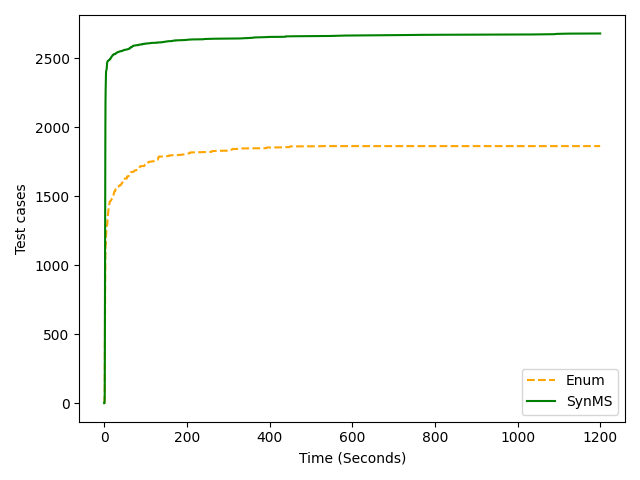
\includegraphics[width=\textwidth]{fig/normal-wythoff-f.png}
        \caption{Comparison on synthesizing winning formulas on the whole benchmark}
    \end{subfigure}
    \begin{subfigure}[b]{0.49\textwidth}
        \centering
        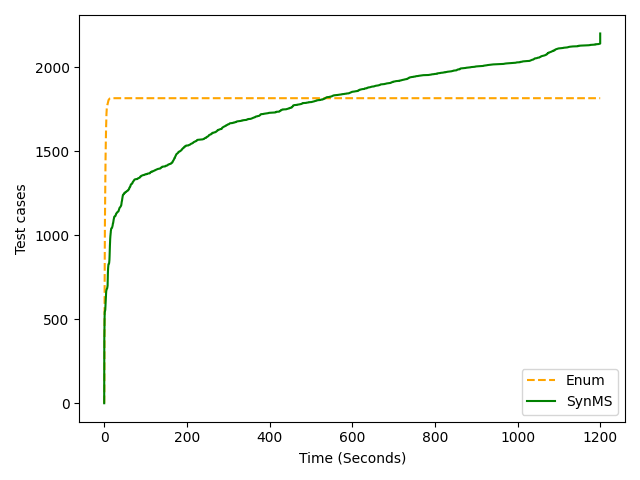
\includegraphics[width=\textwidth]{fig/normal-wythoff-s.png}
        \caption{Comparison on synthesizing winning strategies on the whole benchmark}
    \end{subfigure}
    \caption{Comparison of the running time of synthesizing winning formula and strategy for Wythoff game under normal rule}
    \label{fig:normal-wythoff-line}
\end{figure}

\textbf{Comparison on Chomp game.}
Table \ref{tab:normal-chomp-winFormulas} presents the results for synthesizing winning formulas in the Chomp game under the normal rule.
Out of $8$ test cases, SynEnum solves $2$ formula cases, while SynMS solves $3$, with success rates of $25.0\%$ and $37.5\%$, respectively.
Thus SynMS solves $1$ more formula cases than SynEnum.
The average formula synthesis time is $1.40$ seconds for SynEnum and $4.46$ seconds for SynMS.
Table \ref{tab:normal-chomp-winStrategies} summarizes the corresponding results for synthesizing winning strategies.
SynEnum solves $2$ strategy cases, whereas SynMS solves $2$ strategy cases.
This gives SynMS an advantage of $0$ strategy cases in this benchmark group.
The average strategy synthesis time is $2.26$ seconds for SynEnum and $5.26$ seconds for SynMS.
In terms of solution size, SynEnum produces smaller formulas and strategies on average, with average sizes $4.00$ and $9.50$, while SynMS has average sizes $42.00$ and $10.00$.
Figure \ref{fig:normal-chomp-line} shows the cumulative number of solved test cases over time after filtering the summary data according to the latest Sheet1 counts.

\begin{table*}[h!]
	%字体大小和行距
	\footnotesize
	%列距
	\setlength{\tabcolsep}{3pt}
	\centering
	\begin{tabular}{|c|c|c|c|c|c|c|c|}
		\hline
		\multirow{3}{*}{Category} & \multirow{3}*{\tabincell{c}{Test \\ cases}} & \multicolumn{6}{c|}{Formula}  \\ \cline{3-8} &  & \multicolumn{2}{c|}{Solved} & \multicolumn{2}{c|}{Time} & \multicolumn{2}{c|}{Size} \\ \cline{3-8} & & \multicolumn{1}{c|}{SynEnum} & \multicolumn{1}{c|}{SynMS} & \multicolumn{1}{c|}{SynEnum} & \multicolumn{1}{c|}{SynMS} & \multicolumn{1}{c|}{SynEnum} & SynMS \\ \hline
		Chomp & 7 & 1 & \textbf{2} & \textbf{1.21} & 5.93 & \textbf{4.00} & 61.50 \\ \hline
		L-shaped Chomp & 1 & \textbf{1} & \textbf{1} & 1.59 & \textbf{1.53} & 4.00 & \textbf{3.00} \\ \hline
		Total & 8 & 2 & \textbf{3} & \textbf{1.40} & 4.46 & \textbf{4.00} & 42.00 \\ \hline
	\end{tabular}
	\caption{Results of synthesizing winning formulas for Chomp games under normal rule}
	\label{tab:normal-chomp-winFormulas}
\end{table*}

\begin{table*}[h!]
	%字体大小和行距
	\footnotesize
	%列距
	\setlength{\tabcolsep}{3pt}
	\centering
	\begin{tabular}{|c|c|c|c|c|c|c|c|}
		\hline
		\multirow{3}{*}{Category} & \multirow{3}*{\tabincell{c}{Test \\ cases}} & \multicolumn{6}{c|}{Strategy}  \\ \cline{3-8} &  & \multicolumn{2}{c|}{Solved} & \multicolumn{2}{c|}{Time} & \multicolumn{2}{c|}{Size} \\ \cline{3-8} & & \multicolumn{1}{c|}{SynEnum} & \multicolumn{1}{c|}{SynMS} & \multicolumn{1}{c|}{SynEnum} & \multicolumn{1}{c|}{SynMS} & \multicolumn{1}{c|}{SynEnum} & SynMS \\ \hline
		Chomp & 7 & \textbf{1} & \textbf{1} & \textbf{3.57} & 10.47 & \textbf{9.00} & 10.00 \\ \hline
		L-shaped Chomp & 1 & \textbf{1} & \textbf{1} & 0.96 & \textbf{0.04} & \textbf{10.00} & \textbf{10.00} \\ \hline
		Total & 8 & \textbf{2} & \textbf{2} & \textbf{2.26} & 5.26 & \textbf{9.50} & 10.00 \\ \hline
	\end{tabular}
	\caption{Results of synthesizing winning strategies for Chomp games under normal rule}
	\label{tab:normal-chomp-winStrategies}
\end{table*}

\begin{figure}[h!]
    \centering
    \begin{subfigure}[b]{0.49\textwidth}
        \centering
        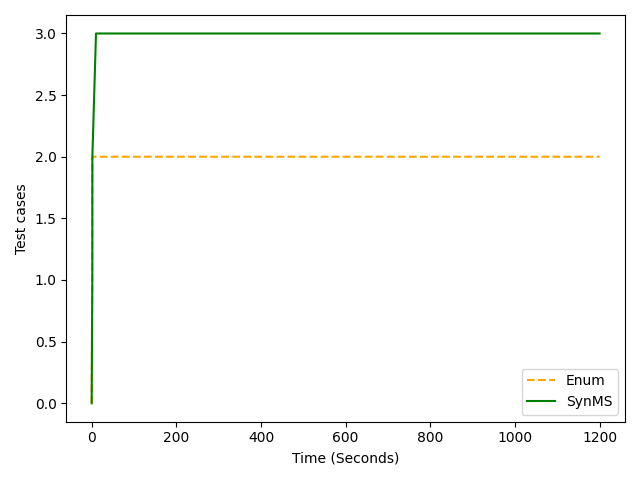
\includegraphics[width=\textwidth]{fig/normal-chomp-f.png}
        \caption{Comparison on synthesizing winning formulas on the whole benchmark}
    \end{subfigure}
    \begin{subfigure}[b]{0.49\textwidth}
        \centering
        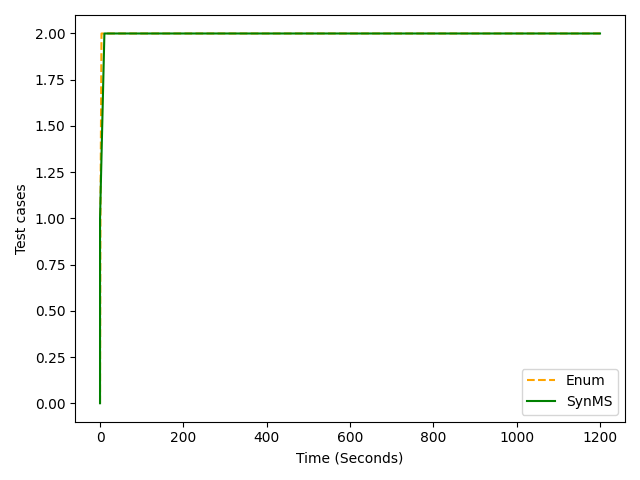
\includegraphics[width=\textwidth]{fig/normal-chomp-s.png}
        \caption{Comparison on synthesizing winning strategies on the whole benchmark}
    \end{subfigure}
    \caption{Comparison of the running time of synthesizing winning formula and strategy for Chomp game under normal rule}
    \label{fig:normal-chomp-line}
\end{figure}

\subsubsection{Experimental Results under mis\`{e}re rule}

\textbf{Comparison on Subtraction game.}
Table \ref{tab:misere-sub-winFormulas} presents the results for synthesizing winning formulas in the Subtraction game under the mis\`{e}re rule.
Out of $479$ test cases, SynEnum solves $178$ formula cases, while SynMS solves $466$, with success rates of $37.2\%$ and $97.3\%$, respectively.
Thus SynMS solves $288$ more formula cases than SynEnum.
The average formula synthesis time is $16.10$ seconds for SynEnum and $17.91$ seconds for SynMS.
Table \ref{tab:misere-sub-winStrategies} summarizes the corresponding results for synthesizing winning strategies.
SynEnum solves $176$ strategy cases, whereas SynMS solves $466$ strategy cases.
This gives SynMS an advantage of $290$ strategy cases in this benchmark group.
The average strategy synthesis time is $1.29$ seconds for SynEnum and $3.62$ seconds for SynMS.
In terms of solution size, SynEnum produces smaller formulas and strategies on average, with average sizes $13.83$ and $62.61$, while SynMS has average sizes $35.81$ and $133.66$.
Figure \ref{fig:misere-sub-line} shows the cumulative number of solved test cases over time after filtering the summary data according to the latest Sheet1 counts.

\begin{table*}[h!]
	%字体大小和行距
	\footnotesize
	%列距
	\setlength{\tabcolsep}{2pt}
	\centering
	\begin{tabular}{|c|c|c|c|c|c|c|c|}
		\hline
		\multirow{3}{*}{Category} & \multirow{3}*{\tabincell{c}{Test \\ cases}} & \multicolumn{6}{c|}{Formula}  \\ \cline{3-8} &  & \multicolumn{2}{c|}{Solved} & \multicolumn{2}{c|}{Time} & \multicolumn{2}{c|}{Size} \\ \cline{3-8} & & \multicolumn{1}{c|}{SynEnum} & \multicolumn{1}{c|}{SynMS} & \multicolumn{1}{c|}{SynEnum} & \multicolumn{1}{c|}{SynMS} & \multicolumn{1}{c|}{SynEnum} & SynMS \\ \hline
		Take-away & 30 & \textbf{30} & \textbf{30} & \textbf{5.13} & 5.82 & \textbf{3.00} & \textbf{3.00} \\ \hline
		Subtraction & 385 & 96 & \textbf{382} & 19.18 & \textbf{8.40} & \textbf{16.25} & 41.63 \\ \hline
		$S,D$-Mark & 64 & 52 & \textbf{54} & \textbf{0.74} & 91.90 & \textbf{3.00} & 12.83 \\ \hline
		Total & 479 & 178 & \textbf{466} & \textbf{16.10} & 17.91 & \textbf{13.83} & 35.81 \\ \hline
	\end{tabular}
	\caption{Results of synthesizing winning formulas for Sub games under mis\`{e}re rule}
	\label{tab:misere-sub-winFormulas}
\end{table*}

\begin{table*}[h!]
	%字体大小和行距
	\footnotesize
	%列距
	\setlength{\tabcolsep}{2pt}
	\centering
	\begin{tabular}{|c|c|c|c|c|c|c|c|}
		\hline
		\multirow{3}{*}{Category} & \multirow{3}*{\tabincell{c}{Test \\ cases}} & \multicolumn{6}{c|}{Strategy}  \\ \cline{3-8} &  & \multicolumn{2}{c|}{Solved} & \multicolumn{2}{c|}{Time} & \multicolumn{2}{c|}{Size} \\ \cline{3-8} & & \multicolumn{1}{c|}{SynEnum} & \multicolumn{1}{c|}{SynMS} & \multicolumn{1}{c|}{SynEnum} & \multicolumn{1}{c|}{SynMS} & \multicolumn{1}{c|}{SynEnum} & SynMS \\ \hline
		Take-away & 30 & \textbf{30} & \textbf{30} & 10.64 & \textbf{8.14} & \textbf{93.00} & \textbf{93.00} \\ \hline
		Subtraction & 385 & 94 & \textbf{382} & \textbf{0.66} & 0.94 & \textbf{64.90} & 149.31 \\ \hline
		$S,D$-Mark & 64 & 52 & \textbf{54} & \textbf{0.32} & 20.08 & \textbf{29.08} & 45.52 \\ \hline
		Total & 479 & 176 & \textbf{466} & \textbf{1.29} & 3.62 & \textbf{62.61} & 133.66 \\ \hline
	\end{tabular}
	\caption{Results of synthesizing winning strategies for Sub games under mis\`{e}re rule}
	\label{tab:misere-sub-winStrategies}
\end{table*}

\begin{figure}[h!]
    \centering
    \begin{subfigure}[b]{0.49\textwidth}
        \centering
        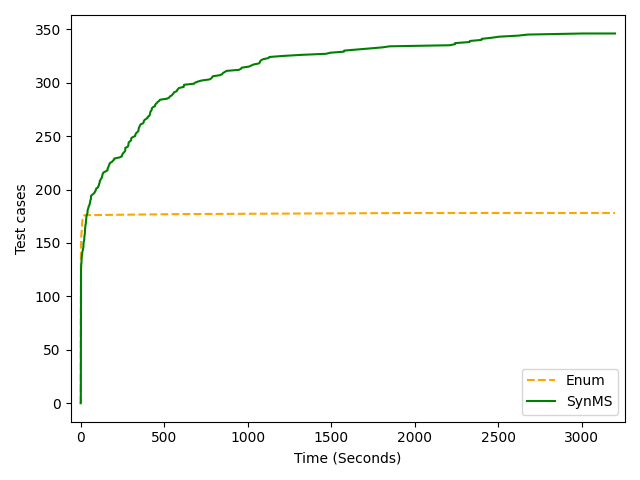
\includegraphics[width=\textwidth]{fig/misere-sub-f.png}
        \caption{Comparison on synthesizing winning formulas on the whole benchmark}
    \end{subfigure}
    \begin{subfigure}[b]{0.49\textwidth}
        \centering
        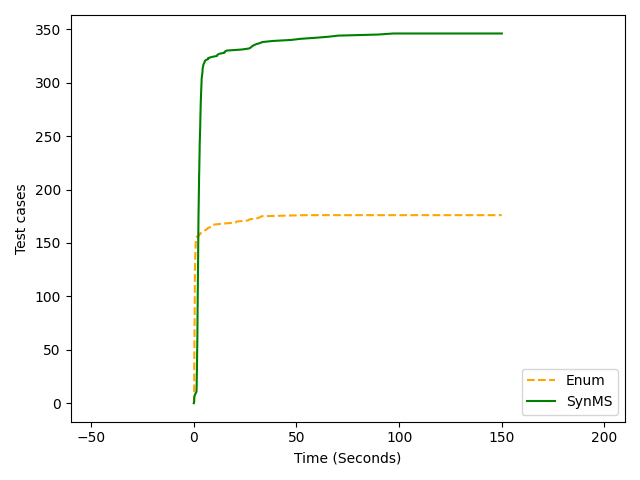
\includegraphics[width=\textwidth]{fig/misere-sub-s.png}
        \caption{Comparison on synthesizing winning strategies on the whole benchmark}
    \end{subfigure}
    \caption{Comparison of the running time of synthesizing winning formula and strategy for Subtraction game under mis\`{e}re rule}
    \label{fig:misere-sub-line}
\end{figure}

\textbf{Comparison on Nim game.}
Table \ref{tab:misere-nim-winFormulas} presents the results for synthesizing winning formulas in the Nim game under the mis\`{e}re rule.
Out of $302$ test cases, SynEnum solves $38$ formula cases, while SynMS solves $85$, with success rates of $12.6\%$ and $28.1\%$, respectively.
Thus SynMS solves $47$ more formula cases than SynEnum.
The average formula synthesis time is $39.69$ seconds for SynEnum and $22.51$ seconds for SynMS.
Table \ref{tab:misere-nim-winStrategies} summarizes the corresponding results for synthesizing winning strategies.
SynEnum solves $36$ strategy cases, whereas SynMS solves $70$ strategy cases.
This gives SynMS an advantage of $34$ strategy cases in this benchmark group.
The average strategy synthesis time is $27.04$ seconds for SynEnum and $203.15$ seconds for SynMS.
In terms of solution size, SynEnum produces smaller formulas and strategies on average, with average sizes $7.05$ and $28.31$, while SynMS has average sizes $165.26$ and $2069.77$.
Figure \ref{fig:misere-nim-line} shows the cumulative number of solved test cases over time after filtering the summary data according to the latest Sheet1 counts.

\begin{table*}[h!]
	%字体大小和行距
	\scriptsize
	%列距
	\setlength{\tabcolsep}{1pt}
	\centering
	\begin{tabular}{|c|c|c|c|c|c|c|c|}
		\hline
		\multirow{3}{*}{Category} & \multirow{3}*{\tabincell{c}{Test \\ cases}} & \multicolumn{6}{c|}{Formula}  \\ \cline{3-8} &  & \multicolumn{2}{c|}{Solved} & \multicolumn{2}{c|}{Time} & \multicolumn{2}{c|}{Size} \\ \cline{3-8} & & \multicolumn{1}{c|}{SynEnum} & \multicolumn{1}{c|}{SynMS} & \multicolumn{1}{c|}{SynEnum} & \multicolumn{1}{c|}{SynMS} & \multicolumn{1}{c|}{SynEnum} & SynMS \\ \hline
		Nim & 7 & \textbf{1} & \textbf{1} & 5.51 & \textbf{1.36} & \textbf{9.00} & 28.00 \\ \hline
		Monotonic Nim & 7 & 4 & \textbf{5} & 126.91 & \textbf{77.54} & \textbf{8.00} & 26.80 \\ \hline
		Empty and Transfer & 7 & 0 & \textbf{1} & - & 2.46 & - & 70.00 \\ \hline
		Empty All But One & 6 & 0 & 0 & - & - & - & - \\ \hline
		Empty and Redistribute & 6 & 0 & \textbf{2} & - & 1.58 & - & 132.00 \\ \hline
		Entropy Reduction Game & 7 & 0 & \textbf{1} & - & 13.56 & - & 36.00 \\ \hline
		Min Game & 6 & 1 & \textbf{4} & \textbf{3.42} & 46.58 & \textbf{6.00} & 249.25 \\ \hline
		$l$-Slow Nim & 180 & 7 & \textbf{15} & \textbf{1.36} & 70.67 & \textbf{4.71} & 190.73 \\ \hline
		Sharing Nim & 7 & \textbf{4} & \textbf{4} & 11.22 & \textbf{7.48} & \textbf{6.50} & 27.00 \\ \hline
		Small Nim & 7 & 2 & \textbf{7} & 92.79 & \textbf{1.65} & 13.50 & \textbf{11.43} \\ \hline
		Greedy Nim & 7 & 2 & \textbf{7} & 103.30 & \textbf{3.34} & \textbf{11.00} & 336.43 \\ \hline
		Odd-or-Even Nim & 7 & 2 & \textbf{5} & 18.96 & \textbf{1.05} & \textbf{8.50} & 377.60 \\ \hline
		Modular Nim & 5 & 1 & \textbf{2} & \textbf{1.25} & 1.53 & \textbf{4.00} & 118.00 \\ \hline
		Pointed Nim & 7 & 0 & \textbf{4} & - & 11.49 & - & 429.50 \\ \hline
		End Nim & 7 & 1 & \textbf{7} & \textbf{2.74} & 3.61 & \textbf{8.00} & 295.00 \\ \hline
		Loop End Nim & 7 & 1 & \textbf{7} & 34.66 & \textbf{9.10} & \textbf{13.00} & 113.57 \\ \hline
		Staircase Nim & 7 & \textbf{7} & \textbf{7} & 64.56 & \textbf{2.56} & \textbf{6.86} & 23.00 \\ \hline
		Circular Nim & 15 & 5 & \textbf{6} & \textbf{3.30} & 5.41 & \textbf{4.60} & 41.83 \\ \hline
		Total & 302 & 38 & \textbf{85} & 39.69 & \textbf{22.51} & \textbf{7.05} & 165.26 \\ \hline
	\end{tabular}
	\caption{Results of synthesizing winning formulas for Nim games under mis\`{e}re rule}
	\label{tab:misere-nim-winFormulas}
\end{table*}

\begin{table*}[h!]
	%字体大小和行距
	\scriptsize
	%列距
	\setlength{\tabcolsep}{1pt}
	\centering
	\begin{tabular}{|c|c|c|c|c|c|c|c|}
		\hline
		\multirow{3}{*}{Category} & \multirow{3}*{\tabincell{c}{Test \\ cases}} & \multicolumn{6}{c|}{Strategy}  \\ \cline{3-8} &  & \multicolumn{2}{c|}{Solved} & \multicolumn{2}{c|}{Time} & \multicolumn{2}{c|}{Size} \\ \cline{3-8} & & \multicolumn{1}{c|}{SynEnum} & \multicolumn{1}{c|}{SynMS} & \multicolumn{1}{c|}{SynEnum} & \multicolumn{1}{c|}{SynMS} & \multicolumn{1}{c|}{SynEnum} & SynMS \\ \hline
		Nim & 7 & \textbf{1} & \textbf{1} & \textbf{2.08} & 5.13 & \textbf{26.00} & 138.00 \\ \hline
		Monotonic Nim & 7 & 4 & \textbf{5} & \textbf{2.02} & 33.12 & \textbf{34.75} & 642.40 \\ \hline
		Empty and Transfer & 7 & 0 & \textbf{1} & - & 315.57 & - & 52.00 \\ \hline
		Empty All But One & 6 & 0 & 0 & - & - & - & - \\ \hline
		Empty and Redistribute & 6 & 0 & 0 & - & - & - & - \\ \hline
		Entropy Reduction Game & 7 & 0 & 0 & - & - & - & - \\ \hline
		Min Game & 6 & 1 & \textbf{4} & \textbf{0.49} & 66.23 & \textbf{11.00} & 1967.00 \\ \hline
		$l$-Slow Nim & 180 & 7 & \textbf{9} & \textbf{0.37} & 0.57 & \textbf{22.00} & 621.78 \\ \hline
		Sharing Nim & 7 & \textbf{3} & 2 & \textbf{0.24} & 16.47 & \textbf{11.33} & 958.00 \\ \hline
		Small Nim & 7 & 2 & \textbf{7} & 1.40 & \textbf{0.85} & \textbf{29.50} & 30.00 \\ \hline
		Greedy Nim & 7 & 2 & \textbf{6} & \textbf{2.01} & 474.69 & \textbf{47.00} & 3101.17 \\ \hline
		Odd-or-Even Nim & 7 & 2 & \textbf{5} & \textbf{0.66} & 190.30 & \textbf{22.50} & 1859.20 \\ \hline
		Modular Nim & 5 & 1 & \textbf{2} & \textbf{0.54} & 25.18 & \textbf{14.00} & 267.00 \\ \hline
		Pointed Nim & 7 & 0 & \textbf{4} & - & 1004.20 & - & 616.75 \\ \hline
		End Nim & 7 & 1 & \textbf{7} & \textbf{1.25} & 400.59 & \textbf{12.00} & 12199.00 \\ \hline
		Loop End Nim & 7 & 1 & \textbf{6} & \textbf{1.15} & 181.08 & \textbf{16.00} & 1215.33 \\ \hline
		Staircase Nim & 7 & \textbf{7} & \textbf{7} & \textbf{3.39} & 44.26 & \textbf{49.00} & 283.43 \\ \hline
		Circular Nim & 15 & \textbf{4} & \textbf{4} & \textbf{231.20} & 339.47 & \textbf{18.00} & 79.75 \\ \hline
		Total & 302 & 36 & \textbf{70} & \textbf{27.04} & 203.15 & \textbf{28.31} & 2069.77 \\ \hline
	\end{tabular}
	\caption{Results of synthesizing winning strategies for Nim games under mis\`{e}re rule}
	\label{tab:misere-nim-winStrategies}
\end{table*}

\begin{figure}[h!]
    \centering
    \begin{subfigure}[b]{0.49\textwidth}
        \centering
        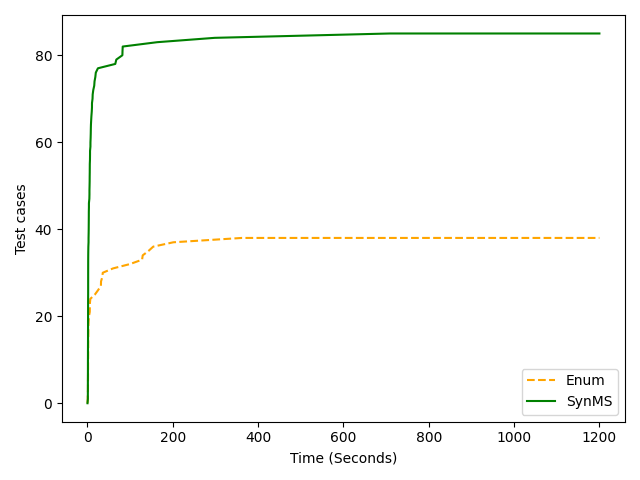
\includegraphics[width=\textwidth]{fig/misere-nim-f.png}
        \caption{Comparison on synthesizing winning formulas on the whole benchmark}
    \end{subfigure}
    \begin{subfigure}[b]{0.49\textwidth}
        \centering
        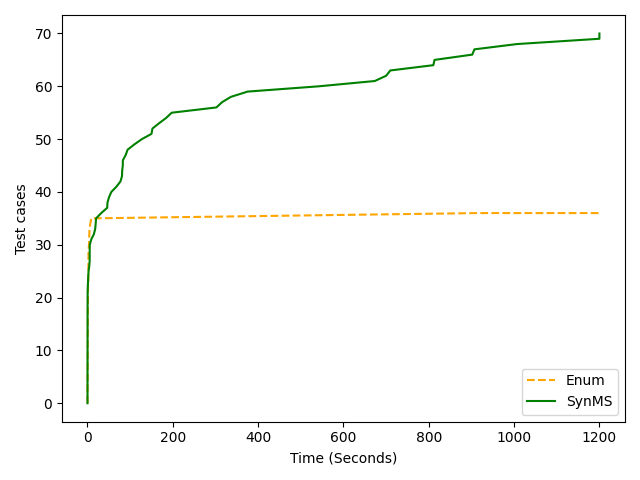
\includegraphics[width=\textwidth]{fig/misere-nim-s.png}
        \caption{Comparison on synthesizing winning strategies on the whole benchmark}
    \end{subfigure}
    \caption{Comparison of the running time of synthesizing winning formula and strategy for Nim game under mis\`{e}re rule}
    \label{fig:misere-nim-line}
\end{figure}

\textbf{Comparison on Welter game.}
Table \ref{tab:misere-welter-winFormulas} presents the results for synthesizing winning formulas in the Welter game under the mis\`{e}re rule.
Out of $7$ test cases, SynEnum solves $2$ formula cases, while SynMS solves $7$, with success rates of $28.6\%$ and $100.0\%$, respectively.
Thus SynMS solves $5$ more formula cases than SynEnum.
The average formula synthesis time is $1.62$ seconds for SynEnum and $158.34$ seconds for SynMS.
Table \ref{tab:misere-welter-winStrategies} summarizes the corresponding results for synthesizing winning strategies.
SynEnum solves $2$ strategy cases, whereas SynMS solves $5$ strategy cases.
This gives SynMS an advantage of $3$ strategy cases in this benchmark group.
The average strategy synthesis time is $0.65$ seconds for SynEnum and $7.97$ seconds for SynMS.
In terms of solution size, SynEnum produces smaller formulas and strategies on average, with average sizes $4.50$ and $43.00$, while SynMS has average sizes $263.14$ and $535.60$.
Figure \ref{fig:misere-welter-line} shows the cumulative number of solved test cases over time after filtering the summary data according to the latest Sheet1 counts.

\begin{table*}[h!]
	%字体大小和行距
	\footnotesize
	%列距
	\setlength{\tabcolsep}{3pt}
	\centering
	\begin{tabular}{|c|c|c|c|c|c|c|c|}
		\hline
		\multirow{3}{*}{Category} & \multirow{3}*{\tabincell{c}{Test \\ cases}} & \multicolumn{6}{c|}{Formula}  \\ \cline{3-8} &  & \multicolumn{2}{c|}{Solved} & \multicolumn{2}{c|}{Time} & \multicolumn{2}{c|}{Size} \\ \cline{3-8} & & \multicolumn{1}{c|}{SynEnum} & \multicolumn{1}{c|}{SynMS} & \multicolumn{1}{c|}{SynEnum} & \multicolumn{1}{c|}{SynMS} & \multicolumn{1}{c|}{SynEnum} & SynMS \\ \hline
		Welter & 1 & 0 & \textbf{1} & - & 1.89 & - & 570.00 \\ \hline
		$l$-Welter & 5 & 2 & \textbf{5} & \textbf{1.62} & 221.01 & \textbf{4.50} & 240.00 \\ \hline
		Max-Welter & 1 & 0 & \textbf{1} & - & 1.48 & - & 72.00 \\ \hline
		Total & 7 & 2 & \textbf{7} & \textbf{1.62} & 158.34 & \textbf{4.50} & 263.14 \\ \hline
	\end{tabular}
	\caption{Results of synthesizing winning formulas for Welter games under mis\`{e}re rule}
	\label{tab:misere-welter-winFormulas}
\end{table*}

\begin{table*}[h!]
	%字体大小和行距
	\footnotesize
	%列距
	\setlength{\tabcolsep}{3pt}
	\centering
	\begin{tabular}{|c|c|c|c|c|c|c|c|}
		\hline
		\multirow{3}{*}{Category} & \multirow{3}*{\tabincell{c}{Test \\ cases}} & \multicolumn{6}{c|}{Strategy}  \\ \cline{3-8} &  & \multicolumn{2}{c|}{Solved} & \multicolumn{2}{c|}{Time} & \multicolumn{2}{c|}{Size} \\ \cline{3-8} & & \multicolumn{1}{c|}{SynEnum} & \multicolumn{1}{c|}{SynMS} & \multicolumn{1}{c|}{SynEnum} & \multicolumn{1}{c|}{SynMS} & \multicolumn{1}{c|}{SynEnum} & SynMS \\ \hline
		Welter & 1 & 0 & \textbf{1} & - & 32.12 & - & 190.00 \\ \hline
		$l$-Welter & 5 & 2 & \textbf{3} & \textbf{0.65} & 0.73 & \textbf{43.00} & 817.33 \\ \hline
		Max-Welter & 1 & 0 & \textbf{1} & - & 5.57 & - & 36.00 \\ \hline
		Total & 7 & 2 & \textbf{5} & \textbf{0.65} & 7.97 & \textbf{43.00} & 535.60 \\ \hline
	\end{tabular}
	\caption{Results of synthesizing winning strategies for Welter games under mis\`{e}re rule}
	\label{tab:misere-welter-winStrategies}
\end{table*}

\begin{figure}[h!]
    \centering
    \begin{subfigure}[b]{0.49\textwidth}
        \centering
        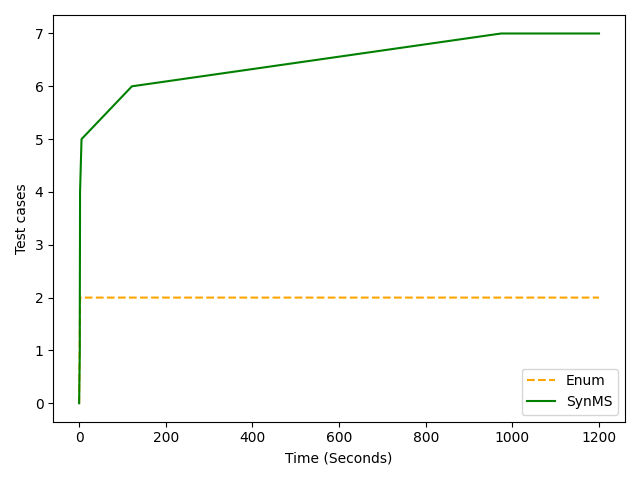
\includegraphics[width=\textwidth]{fig/misere-welter-f.png}
        \caption{Comparison on synthesizing winning formulas on the whole benchmark}
    \end{subfigure}
    \begin{subfigure}[b]{0.49\textwidth}
        \centering
        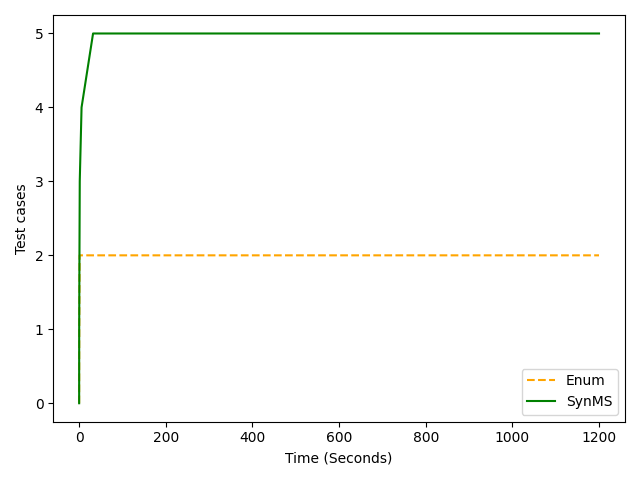
\includegraphics[width=\textwidth]{fig/misere-welter-s.png}
        \caption{Comparison on synthesizing winning strategies on the whole benchmark}
    \end{subfigure}
    \caption{Comparison of the running time of synthesizing winning formula and strategy for Welter game under mis\`{e}re rule}
    \label{fig:misere-welter-line}
\end{figure}

\textbf{Comparison on Wythoff game.}
Table \ref{tab:misere-wythoff-winFormulas} presents the results for synthesizing winning formulas in the Wythoff game under the mis\`{e}re rule.
Out of $2924$ test cases, SynEnum solves $1933$ formula cases, while SynMS solves $2691$, with success rates of $66.1\%$ and $92.0\%$, respectively.
Thus SynMS solves $758$ more formula cases than SynEnum.
The average formula synthesis time is $37.54$ seconds for SynEnum and $27.52$ seconds for SynMS.
Table \ref{tab:misere-wythoff-winStrategies} summarizes the corresponding results for synthesizing winning strategies.
SynEnum solves $1919$ strategy cases, whereas SynMS solves $2420$ strategy cases.
This gives SynMS an advantage of $501$ strategy cases in this benchmark group.
The average strategy synthesis time is $4.62$ seconds for SynEnum and $386.13$ seconds for SynMS.
In terms of solution size, SynEnum produces smaller formulas and strategies on average, with average sizes $6.73$ and $42.68$, while SynMS has average sizes $72.72$ and $453.61$.
Figure \ref{fig:misere-wythoff-line} shows the cumulative number of solved test cases over time after filtering the summary data according to the latest Sheet1 counts.

\begin{table*}[h!]
	%字体大小和行距
	\fontsize{4}{8}
	\selectfont
	%列距
	\setlength{\tabcolsep}{0.8pt}
	\centering
	\begin{tabular}{|c|c|c|c|c|c|c|c|}
		\hline
		\multirow{3}{*}{Category} & \multirow{3}*{\tabincell{c}{Test \\ cases}} & \multicolumn{6}{c|}{Formula}  \\ \cline{3-8} &  & \multicolumn{2}{c|}{Solved} & \multicolumn{2}{c|}{Time} & \multicolumn{2}{c|}{Size} \\ \cline{3-8} & & \multicolumn{1}{c|}{SynEnum} & \multicolumn{1}{c|}{SynMS} & \multicolumn{1}{c|}{SynEnum} & \multicolumn{1}{c|}{SynMS} & \multicolumn{1}{c|}{SynEnum} & SynMS \\ \hline
		Wythoff & 21 & 10 & \textbf{19} & 41.51 & \textbf{2.57} & \textbf{6.60} & 152.95 \\ \hline
		$l$-Wythoff & 140 & 80 & \textbf{123} & 48.85 & \textbf{46.97} & \textbf{7.21} & 75.62 \\ \hline
		Monotonic $l$-Diet Wythoff & 105 & 61 & \textbf{104} & 31.07 & \textbf{11.34} & \textbf{5.28} & 66.65 \\ \hline
		Wythoff with subtraction set $S$ & 315 & 200 & \textbf{287} & 24.59 & \textbf{4.75} & \textbf{6.28} & 106.17 \\ \hline
		Wythoff with a function $f$ & 168 & 116 & \textbf{153} & 38.93 & \textbf{6.13} & \textbf{7.37} & 63.46 \\ \hline
		1st($l_1$,$l_2$)\-restricted Wythoff & 315 & 214 & \textbf{285} & 26.60 & \textbf{2.26} & \textbf{6.83} & 99.46 \\ \hline
		2nd($l_1$,$l_2$)\-restricted Wythoff & 600 & 440 & \textbf{600} & 37.98 & \textbf{2.80} & \textbf{6.36} & 59.01 \\ \hline
		3rd($l_1$,$l_2$)\-restricted Wythoff & 700 & 404 & \textbf{588} & \textbf{55.56} & 96.15 & \textbf{7.18} & 54.75 \\ \hline
		4th($l_1$,$l_2$)\-restricted Wythoff & 560 & 408 & \textbf{532} & 29.58 & \textbf{11.05} & \textbf{6.80} & 76.01 \\ \hline
		Total & 2924 & 1933 & \textbf{2691} & 37.54 & \textbf{27.52} & \textbf{6.73} & 72.72 \\ \hline
	\end{tabular}
	\caption{Results of synthesizing winning formulas for Wythoff games under mis\`{e}re rule}
	\label{tab:misere-wythoff-winFormulas}
\end{table*}

\begin{table*}[h!]
	%字体大小和行距
	\fontsize{4}{8}
	\selectfont
	%列距
	\setlength{\tabcolsep}{0.8pt}
	\centering
	\begin{tabular}{|c|c|c|c|c|c|c|c|}
		\hline
		\multirow{3}{*}{Category} & \multirow{3}*{\tabincell{c}{Test \\ cases}} & \multicolumn{6}{c|}{Strategy}  \\ \cline{3-8} &  & \multicolumn{2}{c|}{Solved} & \multicolumn{2}{c|}{Time} & \multicolumn{2}{c|}{Size} \\ \cline{3-8} & & \multicolumn{1}{c|}{SynEnum} & \multicolumn{1}{c|}{SynMS} & \multicolumn{1}{c|}{SynEnum} & \multicolumn{1}{c|}{SynMS} & \multicolumn{1}{c|}{SynEnum} & SynMS \\ \hline
		Wythoff & 21 & 10 & \textbf{16} & \textbf{1.56} & 21.65 & \textbf{31.40} & 278.56 \\ \hline
		$l$-Wythoff & 140 & 80 & \textbf{102} & \textbf{5.62} & 663.64 & \textbf{54.11} & 790.93 \\ \hline
		Monotonic $l$-Diet Wythoff & 105 & 61 & \textbf{95} & \textbf{0.44} & 0.50 & \textbf{22.03} & 419.32 \\ \hline
		Wythoff with subtraction set $S$ & 315 & 200 & \textbf{266} & \textbf{1.70} & 25.91 & \textbf{30.09} & 368.59 \\ \hline
		Wythoff with a function $f$ & 168 & 116 & \textbf{140} & \textbf{3.54} & 442.66 & \textbf{52.01} & 598.21 \\ \hline
		1st($l_1$,$l_2$)\-restricted Wythoff & 315 & 214 & \textbf{264} & \textbf{2.38} & 16.59 & \textbf{37.33} & 365.79 \\ \hline
		2nd($l_1$,$l_2$)\-restricted Wythoff & 600 & 440 & \textbf{538} & \textbf{2.52} & 705.10 & \textbf{43.83} & 328.33 \\ \hline
		3rd($l_1$,$l_2$)\-restricted Wythoff & 700 & 404 & \textbf{499} & \textbf{12.26} & 723.65 & \textbf{59.64} & 562.53 \\ \hline
		4th($l_1$,$l_2$)\-restricted Wythoff & 560 & 394 & \textbf{500} & \textbf{2.70} & 105.31 & \textbf{31.73} & 474.15 \\ \hline
		Total & 2924 & 1919 & \textbf{2420} & \textbf{4.62} & 386.13 & \textbf{42.68} & 453.61 \\ \hline
	\end{tabular}
	\caption{Results of synthesizing winning strategies for Wythoff games under mis\`{e}re rule}
	\label{tab:misere-wythoff-winStrategies}
\end{table*}

\begin{figure}[h!]
    \centering
    \begin{subfigure}[b]{0.49\textwidth}
        \centering
        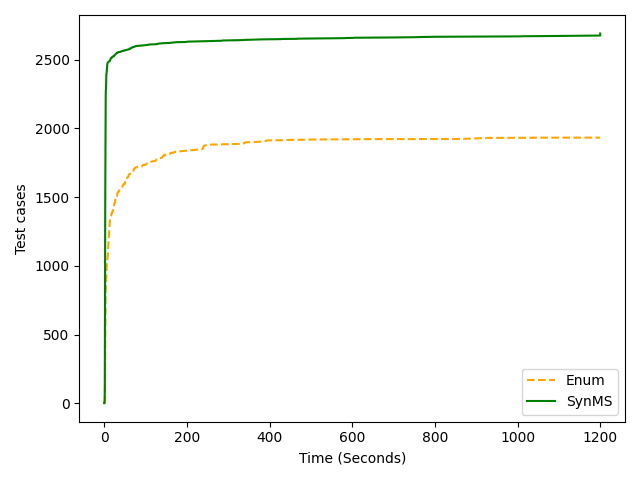
\includegraphics[width=\textwidth]{fig/misere-wythoff-f.png}
        \caption{Comparison on synthesizing winning formulas on the whole benchmark}
    \end{subfigure}
    \begin{subfigure}[b]{0.49\textwidth}
        \centering
        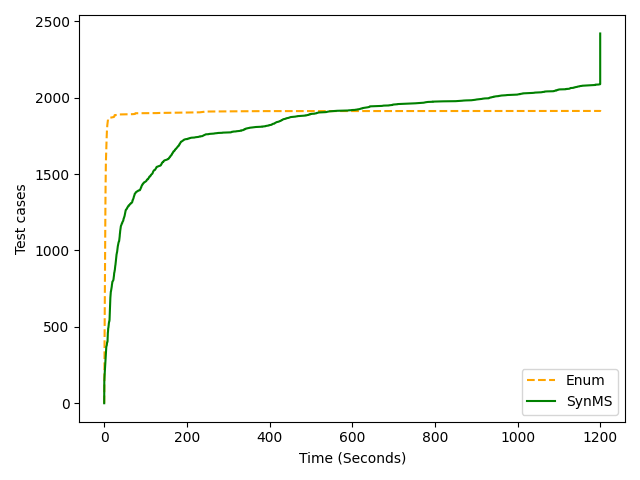
\includegraphics[width=\textwidth]{fig/misere-wythoff-s.png}
        \caption{Comparison on synthesizing winning strategies on the whole benchmark}
    \end{subfigure}
    \caption{Comparison of the running time of synthesizing winning formula and strategy for Wythoff game under mis\`{e}re rule}
    \label{fig:misere-wythoff-line}
\end{figure}

\textbf{Comparison on Chomp game.}
Table \ref{tab:misere-chomp-winFormulas} presents the results for synthesizing winning formulas in the Chomp game under the mis\`{e}re rule.
Out of $8$ test cases, SynEnum solves $2$ formula cases, while SynMS solves $3$, with success rates of $25.0\%$ and $37.5\%$, respectively.
Thus SynMS solves $1$ more formula cases than SynEnum.
The average formula synthesis time is $17.48$ seconds for SynEnum and $4.66$ seconds for SynMS.
Table \ref{tab:misere-chomp-winStrategies} summarizes the corresponding results for synthesizing winning strategies.
SynEnum solves $2$ strategy cases, whereas SynMS solves $2$ strategy cases.
This gives SynMS an advantage of $0$ strategy cases in this benchmark group.
The average strategy synthesis time is $3.33$ seconds for SynEnum and $5.17$ seconds for SynMS.
In terms of solution size, SynEnum produces smaller formulas on average, while SynMS produces smaller strategies in this group.
Figure \ref{fig:misere-chomp-line} shows the cumulative number of solved test cases over time after filtering the summary data according to the latest Sheet1 counts.

\begin{table*}[h!]
	%字体大小和行距
	\footnotesize
	%列距
	\setlength{\tabcolsep}{3pt}
	\centering
	\begin{tabular}{|c|c|c|c|c|c|c|c|}
		\hline
		\multirow{3}{*}{Category} & \multirow{3}*{\tabincell{c}{Test \\ cases}} & \multicolumn{6}{c|}{Formula}  \\ \cline{3-8} &  & \multicolumn{2}{c|}{Solved} & \multicolumn{2}{c|}{Time} & \multicolumn{2}{c|}{Size} \\ \cline{3-8} & & \multicolumn{1}{c|}{SynEnum} & \multicolumn{1}{c|}{SynMS} & \multicolumn{1}{c|}{SynEnum} & \multicolumn{1}{c|}{SynMS} & \multicolumn{1}{c|}{SynEnum} & SynMS \\ \hline
		Chomp & 7 & 1 & \textbf{2} & \textbf{1.49} & 6.09 & \textbf{3.00} & 79.50 \\ \hline
		L-shaped Chomp & 1 & \textbf{1} & \textbf{1} & 33.46 & \textbf{1.81} & \textbf{9.00} & 28.00 \\ \hline
		Total & 8 & 2 & \textbf{3} & 17.48 & \textbf{4.66} & \textbf{6.00} & 62.33 \\ \hline
	\end{tabular}
	\caption{Results of synthesizing winning formulas for Chomp games under mis\`{e}re rule}
	\label{tab:misere-chomp-winFormulas}
\end{table*}

\begin{table*}[h!]
	%字体大小和行距
	\footnotesize
	%列距
	\setlength{\tabcolsep}{3pt}
	\centering
	\begin{tabular}{|c|c|c|c|c|c|c|c|}
		\hline
		\multirow{3}{*}{Category} & \multirow{3}*{\tabincell{c}{Test \\ cases}} & \multicolumn{6}{c|}{Strategy}  \\ \cline{3-8} &  & \multicolumn{2}{c|}{Solved} & \multicolumn{2}{c|}{Time} & \multicolumn{2}{c|}{Size} \\ \cline{3-8} & & \multicolumn{1}{c|}{SynEnum} & \multicolumn{1}{c|}{SynMS} & \multicolumn{1}{c|}{SynEnum} & \multicolumn{1}{c|}{SynMS} & \multicolumn{1}{c|}{SynEnum} & SynMS \\ \hline
		Chomp & 7 & \textbf{1} & \textbf{1} & \textbf{5.28} & 7.79 & 65.00 & \textbf{14.00} \\ \hline
		L-shaped Chomp & 1 & \textbf{1} & \textbf{1} & \textbf{1.38} & 2.54 & \textbf{26.00} & 34.00 \\ \hline
		Total & 8 & \textbf{2} & \textbf{2} & \textbf{3.33} & 5.17 & 45.50 & \textbf{24.00} \\ \hline
	\end{tabular}
	\caption{Results of synthesizing winning strategies for Chomp games under mis\`{e}re rule}
	\label{tab:misere-chomp-winStrategies}
\end{table*}

\begin{figure}[h!]
    \centering
    \begin{subfigure}[b]{0.49\textwidth}
        \centering
        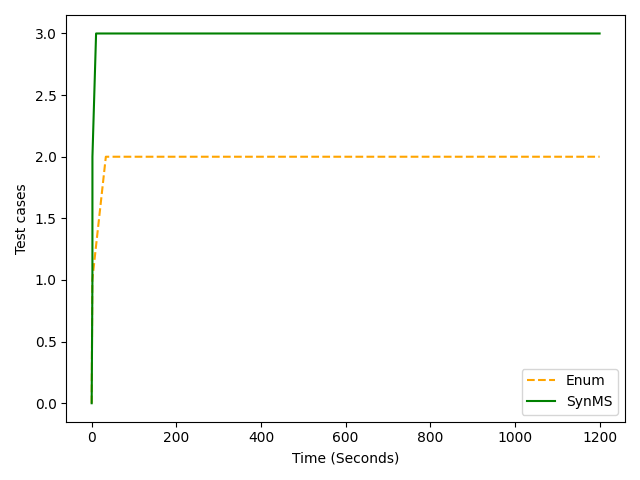
\includegraphics[width=\textwidth]{fig/misere-chomp-f.png}
        \caption{Comparison on synthesizing winning formulas on the whole benchmark}
    \end{subfigure}
    \begin{subfigure}[b]{0.49\textwidth}
        \centering
        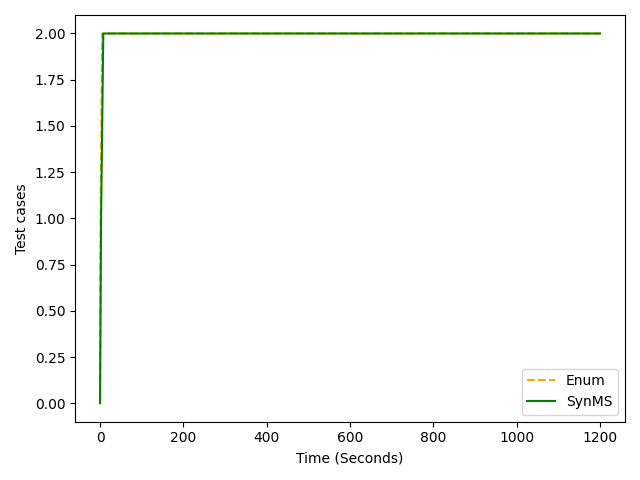
\includegraphics[width=\textwidth]{fig/misere-chomp-s.png}
        \caption{Comparison on synthesizing winning strategies on the whole benchmark}
    \end{subfigure}
    \caption{Comparison of the running time of synthesizing winning formula and strategy for Chomp game under mis\`{e}re rule}
    \label{fig:misere-chomp-line}
\end{figure}

